
%%%%%%%%%%%%%%%%%%%%%%%%%%%%%%%%%%%%%%%%%%%%%%%%%%%%%%%%%%%%%%%%%%%%%%%%%%%%%%%%%%%%%%%
%%%%%%%%%%%%%%%%%%%%%%%%%%%%%%%%%%%%%%%%%%%%%%%%%%%%%%%%%%%%%%%%%%%%%%%%%%%%%%%%%%%%%%%
% 
% This top part of the document is called the 'preamble'.  Modify it with caution!
%
% The real document starts below where it says 'The main document starts here'.

\documentclass[12pt]{article}

\usepackage{amssymb,amsmath,amsthm}
\usepackage[top=1in, bottom=1in, left=1.25in, right=1.25in]{geometry}
\usepackage{fancyhdr}
\usepackage{enumerate}
\usepackage{listings}
\usepackage{graphicx}
\usepackage{float}
\usepackage{multicol}
% Comment the following line to use TeX's default font of Computer Modern.
\usepackage{times,txfonts}
\usepackage{mwe}
\usepackage{caption}
\usepackage{subcaption}

\usepackage{tikz}
\def\checkmark{\tikz\fill[scale=0.4](0,.35) -- (.25,0) -- (1,.7) -- (.25,.15) -- cycle;} 



\makeatletter
\renewcommand*\env@matrix[1][*\c@MaxMatrixCols c]{%
  \hskip -\arraycolsep
  \let\@ifnextchar\new@ifnextchar
  \array{#1}}
\makeatother

\newtheoremstyle{homework}% name of the style to be used
  {18pt}% measure of space to leave above the theorem. E.g.: 3pt
  {12pt}% measure of space to leave below the theorem. E.g.: 3pt
  {}% name of font to use in the body of the theorem
  {}% measure of space to indent
  {\bfseries}% name of head font
  {:}% punctuation between head and body
  {2ex}% space after theorem head; " " = normal interword space
  {}% Manually specify head
\theoremstyle{homework} 

% Set up an Exercise environment and a Solution label.
\newtheorem*{exercisecore}{Exercise \@currentlabel}
\newenvironment{exercise}[1]
{\def\@currentlabel{#1}\exercisecore}
{\endexercisecore}

\newcommand{\localhead}[1]{\par\smallskip\noindent\textbf{#1}\nobreak\\}%
\newcommand\solution{\localhead{Solution:}}

%%%%%%%%%%%%%%%%%%%%%%%%%%%%%%%%%%%%%%%%%%%%%%%%%%%%%%%%%%%%%%%%%%%%%%%%
%
% Stuff for getting the name/document date/title across the header
\makeatletter
\RequirePackage{fancyhdr}
\pagestyle{fancy}
\fancyfoot[C]{\ifnum \value{page} > 1\relax\thepage\fi}
\fancyhead[L]{\ifx\@doclabel\@empty\else\@doclabel\fi}
\fancyhead[C]{\ifx\@docdate\@empty\else\@docdate\fi}
\fancyhead[R]{\ifx\@docauthor\@empty\else\@docauthor\fi}
\headheight 15pt

\def\doclabel#1{\gdef\@doclabel{#1}}
\doclabel{Use {\tt\textbackslash doclabel\{MY LABEL\}}.}
\def\docdate#1{\gdef\@docdate{#1}}
\docdate{Use {\tt\textbackslash docdate\{MY DATE\}}.}
\def\docauthor#1{\gdef\@docauthor{#1}}
\docauthor{Use {\tt\textbackslash docauthor\{MY NAME\}}.}
\makeatother

% Shortcuts for blackboard bold number sets (reals, integers, etc.)
\newcommand{\Reals}{\ensuremath{\mathbb R}}
\newcommand{\Nats}{\ensuremath{\mathbb N}}
\newcommand{\Ints}{\ensuremath{\mathbb Z}}
\newcommand{\Rats}{\ensuremath{\mathbb Q}}
\newcommand{\Cplx}{\ensuremath{\mathbb C}}
%% Some equivalents that some people may prefer.
\let\RR\Reals
\let\NN\Nats
\let\II\Ints
\let\CC\Cplx

%\textbf{Code:}
%\begin{center}
%  \lstinputlisting{NewtonsMethodP5.m}
%\end{center}
%
%\textbf{Console:}
%\begin{center}
%  \lstinputlisting{P5C.txt}
%\end{center}
%\vspace{.15in}


%\begin{figure}[H]
%  \begin{center}
%    \caption{The one-norm unit ball}
%    \includegraphics[width=.76\textwidth]{1norm.png}
%  \end{center}
%\end{figure}




%%%%%%%%%%%%%%%%%%%%%%%%%%%%%%%%%%%%%%%%%%%%%%%%%%%%%%%%%%%%%%%%%%%%%%%%%%%%%%%%%%%%%%%
%%%%%%%%%%%%%%%%%%%%%%%%%%%%%%%%%%%%%%%%%%%%%%%%%%%%%%%%%%%%%%%%%%%%%%%%%%%%%%%%%%%%%%%
% 
% The main document start here.

% The following commands set up the material that appears in the header.
\doclabel{Math 661: Homework 3}
\docauthor{Stefano Fochesatto}
\docdate{\today}


\begin{document}

\begin{exercise}{4.3} Consider the problem, 
  \begin{align*}
    \text{minimize }f(x) = -x_1 &- x_2\\
    \text{subject to }x_1 + x_2 &\leq 2\\
    x_1, x_2 &\geq 0\\
  \end{align*}
  \begin{enumerate}
  \item Consider the feasible directions at $x = (0,0)^T,(0,1)^T, (1,1)^T,$ and $(0,2)^T$. 
  \begin{proof}[Solution]
    Note that $(0, 0)^T$ only makes $x_1, x_2 \geq 0$ active. Therefore the feasible direction $p$ is defined by, 
    \begin{equation*}
      (1, 0)(p_1, p_2)^T = p_1 \geq 0.
    \end{equation*}
    \begin{equation*}
      (0, 1)(p_1, p_2)^T = p_2 \geq 0.
    \end{equation*}
    Note that $(0, 1)^T$ only makes $x_1 \geq 0$ active. Therefore the feasible direction $p$ is defined by, 
    \begin{equation*}
      (1, 0)(p_1, p_2)^T = p_1 \geq 0.
    \end{equation*}
    With $p_2 \in \RR$. 
    Note that $(1,1)^T$ only makes $x_1 + x_2 \leq 2$. Therefore the feasible direction $p$ is defined by, 
    \begin{equation*}
      (-1, -1)(p_1, p_2)^T = -p_1 - p_2 \geq 0.
    \end{equation*}
    Finally note that $(0,2)^T$ makes $x_1 + x_2 \leq 2$ and $x_1 \geq 0$ active. Therefore the feasible direction $p$ is defined by, 
    \begin{equation*}
      (-1, -1)(p_1, p_2) = -p_1 - p_2 \geq 0.
    \end{equation*}
    \begin{equation*}
      (1, 0)(p_1, p_2)^T = p_1 \geq 0.
    \end{equation*}
  \end{proof}
  \vspace{.15in}


  \item Determine whether there exists feasible descent direction at these points, and hence 
  determine which (if any) of the points can be local minimizers.
  \begin{proof}[Solution] Recall that any direction $p$ which satisfies $\nabla f(x)^{T}p < 0$, will be a descent direction.
    Since $f(x)$ is linear know that  $\nabla f(x)^{T} = (-1, -1)$. Computing the inner product with $p$ we get that, 
    \begin{equation*}
      (-1, -1)(p_1, p_2)^T = -p_1 - p_2 < 0. 
    \end{equation*}
    Or rephrased $p_1 + p_2 > 0$. For point $(0, 0)$ with constraints $p_1, p_2 \geq 0$ every non-trivial feasible direction is a descent direction. 
    For point $(0, 1)$ with constraint $p_1 \geq 0$ as long as $p_1 > p_2$ our feasible direction is a descent direction. 
    For point $(1, 1)$ with constraint $p_1 + p_2 \leq 0$ every feasible direction is an ascent direction. 
    For point $(0, 2)$ with constraint $p_1 + p_2 \leq 0$ and $p_1 \geq 0$ every feasible direction is an ascent direction. 
  \end{proof}
\end{enumerate}
\end{exercise}
\vspace{.5in}






\begin{exercise}{6.5} Find the first three terms of the Taylor series for,
  \begin{equation*}
    f(x_1, x_2) = \sqrt{x_1^2 + x_2^2}
  \end{equation*}
  about the point $x_0 = (3, 4)^T$. 
  \begin{proof}[Solution]
    Recall the Multidimensional Taylor Series expansion with cubic remainder, 
    \begin{equation*}
      f(x_0 + p) = f(x_0) + p^T\nabla f(x_0) + \dfrac{1}{2} p^T\nabla^2 f(x_0)p + g(\Xi)
    \end{equation*}
    Where $g$ is some function cubic in $p$ with a tensor shaped $\nabla^3 f(x_0)$ and $ x_0< \Xi < p$ (Book does not go 
    into detail about how this term is notated). Computing $\nabla f(x)$ and $\nabla^2 f(x)$ we get, 
    \begin{equation*}
      \nabla f(x) = 
      \begin{pmatrix}
        \dfrac{x}{\sqrt{x^2+y^2}}\\[17pt]
        \dfrac{y}{\sqrt{x^2+y^2}}
      \end{pmatrix},
    \end{equation*}
    \begin{equation*}
      \nabla^2 f(x) = 
      \begin{pmatrix}
        \dfrac{y^2}{\left(x^2+y^2\right)\sqrt{x^2+y^2}}& -\dfrac{xy}{\left(x^2+y^2\right)^{\frac{3}{2}}}\\[20pt]
        -\dfrac{xy}{\left(x^2+y^2\right)^{\frac{3}{2}}} & \dfrac{x^2}{\left(x^2+y^2\right)\sqrt{x^2+y^2}}
      \end{pmatrix}.
    \end{equation*}
    Plugging in our $x_0 = (3, 4)^T$, we get
    \begin{equation*}
      \nabla f(x_0) = 
      \begin{pmatrix}
        \dfrac{3}{5}\\[10pt]
        \dfrac{3}{5}
      \end{pmatrix},
    \end{equation*}
    \begin{equation*}
      \nabla^2 f(x_0) = 
      \begin{pmatrix}
        \dfrac{16}{125}& -\dfrac{12}{125}\\[10pt]
        -\dfrac{12}{125} & \dfrac{9}{125}
      \end{pmatrix}.
    \end{equation*}
    Finally for some $p = (p_1, p_2)^T$ we get the first three terms of the taylor series are, 
    \begin{equation*}
      f(x_0 + p) \approx 5 + p^T
      \begin{pmatrix}
        \dfrac{3}{5}\\[10pt]
        \dfrac{3}{5}
      \end{pmatrix}
      + \dfrac{1}{2}
      p^{T}
      \begin{pmatrix}
        \dfrac{16}{125}& -\dfrac{12}{125}\\[10pt]
        -\dfrac{12}{125} & \dfrac{9}{125}
      \end{pmatrix}
      p
    \end{equation*}
  \end{proof}
\end{exercise}
\vspace{.5in}




\begin{exercise}{1.1} Find the set of all feasible directions at points $x_a = (0, 0, 2)^T$, $x_b = (3, 0, 1)^T$, and $x_c = (1, 1, 1)^T$ for Example 3.1. The set of constraints from Example 3.1 are, 
  \begin{align*}
    x_1 + 2x_2 + 3x_3 &= 6,\\
    x_1, x_2, x_3, &\geq 0.
  \end{align*}
  \begin{proof}[Solution]
    Recall that $p$ is a feasible direction with respect to the feasible set at a point $x$ if and only if 
    \begin{equation*}
      a_i^Tp = 0, i \in \varepsilon 
    \end{equation*}
    \begin{equation*}
      a_i^Tp \geq 0, i \in \hat{\tau}  
    \end{equation*}
    Where $\varepsilon$ is the set of equality constraints, $\hat{\tau}$ is the set of active inequality constraints, and 
    $a_i$ are the vectors which define our constraints. For our set of constraints, $a_1 = (1, 2, 3)^T$,
    $a_2 = (1, 0, 0)^T$, $a_3 = (0, 1, 0)^T$, $a_4 = (0, 0, 1)^T$.\\\\
    Consider point $x_a = (0, 0, 2)^T$. Note that the only active inequality constraints are $a_2$, and $a_3$. 
    Therefore the following inequalities describe the set of all feasible directions, 
    \begin{equation*}
      a_1^Tp = 1p_1 + 2p_2 + 3p_3 = 0
    \end{equation*}
    and 
    \begin{equation*}
      a_2^Tp = 1p_1 + 0p_2 + 0p_3 = p_1 \geq 0
    \end{equation*}
    \begin{equation*}
      a_3^Tp = 0p_1 + 1p_2 + 0p_3 = p_2 \geq 0.
    \end{equation*}

    Consider the point $x_b = (3, 0, 1)$. Note that the only active inequality constraint is $a_3$. Therefore the following equalities and inequalities describe the set of all feasible directions, 
    \begin{equation*}
      a_1^Tp = 1p_1 + 2p_2 + 3p_3 = 0
    \end{equation*}
    and 
    \begin{equation*}
      a_3^Tp = 0p_1 + 1p_2 + 0p_3 = p_2 \geq 0.
    \end{equation*}

    Consider the point $x_c = (1, 1, 1)^T$. Note that there are no active inequality constraints so we only have to satisfy the equality constraint, 
    \begin{equation*}
      a_1^Tp = 1p_1 + 2p_2 + 3p_3 = 0
    \end{equation*}
  
  \end{proof}
\end{exercise}
\vspace{.5in}





\begin{exercise}{1.3} Consider the system of inequality constraints $Ax \leq b$ with 
  \begin{equation*}
    A = \begin{bmatrix}
      9 & 4 &1 & 9  &-7\\
      6 & -7& 8&  -4& -6\\
      1 & 6 &3 & -7 &6  
    \end{bmatrix}
    \text{    and    }
    b = \begin{bmatrix}
      -15\\
      -30\\
      -20
    \end{bmatrix}
  \end{equation*}
  For the given values of $x$ and $p$, perform a ratio test to determine the maximum step 
  length $\overline{\alpha}$ such that $x + \overline{\alpha}p$ remains feasible. 
  \begin{enumerate}
    \item[\textbf{(i)}] $x = (8, 4, -3, 4, 1)^T$ and $p = (1, 1, 1, 1, 1)^T$
    \begin{proof}[Solution] Evaluating $Ax$ to see which constraints are active/inactive, 
      \begin{equation*}
        \begin{bmatrix}9&4&1&9&-7\\ 6&-7&8&-4&-6\\ 1&6&3&-7&6\end{bmatrix}\begin{pmatrix}8\\ 4\\ -3\\ 4\\ 1\end{pmatrix}=\begin{pmatrix}114\\ -26\\ 1\end{pmatrix}
      \end{equation*} 
      Since each component of our result is strictly greater than $b$ every inequality constraint is inactive.\\\\
      Recall that by the ratio test we know that, 
      \begin{equation*}
        \overline{\alpha} = min\{(a_i^Tx - b_i)/(a_i^Tp): (a_i^Tp) < 0\}
      \end{equation*}
      Computing all $(a_i^Tp)$ or $Ap$ to see which constraints bound our step, 
      \begin{equation*}
        \begin{bmatrix}9&4&1&9&-7\\ 6&-7&8&-4&-6\\ 1&6&3&-7&6\end{bmatrix}\begin{pmatrix}1\\ 1\\ 1\\ 1\\ 1\end{pmatrix}=\begin{pmatrix}16\\ -3\\ 9\end{pmatrix}
      \end{equation*}
      Since $a_2$ is the only constraint which our direction is set to intersect, it defines the $\overline{\alpha}$ in the ratio test, 
      \begin{equation*}
        \overline{\alpha} = ((6, -7, 8, -4, -6)(8, 4, -3, 4, 1)^T + 30)/3 = \frac{4}{3}.
      \end{equation*}
    \end{proof}
    \vspace{.15in}

      \item[\textbf{(ii)}] $x = (7, -4, -3, -3, 3)^T$ and $p = (3, 2, 0, 1, -2)^T$
      \begin{proof}[Solution] Evaluating $Ax$ to see which constraints are active/inactive, 
        \begin{equation*}
        \begin{bmatrix}9&4&1&9&-7\\ 6&-7&8&-4&-6\\ 1&6&3&-7&6\end{bmatrix}\begin{pmatrix}7\\ -4\\ -3\\ -3\\ 3\end{pmatrix}=\begin{pmatrix}-4\\ 40\\ 13\end{pmatrix}
      \end{equation*}
        Since each component of our result is strictly greater than $b$ every inequality constraint is inactive.\\\\
        Computing all $(a_i^Tp)$ or $Ap$ to see which constraints bound our step, 
        \begin{equation*}
          \begin{bmatrix}9&4&1&9&-7\\ 6&-7&8&-4&-6\\ 1&6&3&-7&6\end{bmatrix}\begin{pmatrix}3\\ 2\\ 0\\ 1\\ -2\end{pmatrix}=\begin{pmatrix}58\\ 12\\ -4\end{pmatrix}
        \end{equation*}
        Since $a_3$ is the only constraint which our direction is set to intersect, it defines the $\overline{\alpha}$ in the ratio test, 
        \begin{equation*}
          \overline{\alpha} = (( 1 , 6 , 3 , -7 , 6)(7, -4, -3, -3, 3)^T + 20)/4 = \frac{33}{4}.
        \end{equation*}
      \end{proof}
    \vspace{.15in}

    \item[\textbf{(iii)}] $x = (5, 0, -6, -8, -3)^T$ and $p = (5, 0, 5, 1, 3)^T$
    \begin{proof}[Solution] Evaluating $Ax$ to see which constraints are active/inactive, 
      \begin{equation*}
        \begin{bmatrix}9&4&1&9&-7\\ 6&-7&8&-4&-6\\ 1&6&3&-7&6\end{bmatrix}\begin{pmatrix}5\\ 0\\ -6\\ -8\\ -3\end{pmatrix}=\begin{pmatrix}-12\\ 32\\ 25\end{pmatrix}
    \end{equation*}
      Since each component of our result is strictly greater than $b$ every inequality constraint is inactive.\\\\
      Computing all $(a_i^Tp)$ or $Ap$ to see which constraints bound our step, 
      \begin{equation*}
        \begin{bmatrix}9&4&1&9&-7\\ 6&-7&8&-4&-6\\ 1&6&3&-7&6\end{bmatrix}\begin{pmatrix}5\\ 0\\ 5\\ 1\\ 3\end{pmatrix}=\begin{pmatrix}38\\ 48\\ 31\end{pmatrix}
      \end{equation*}
      Since $(a_i^Tp) \geq 0$ for all constraints $a_i$, $\overline{\alpha}$ is unbounded. 
    \end{proof}
  \vspace{.15in}

  \item[\textbf{(iv)}] $x = (9, 1, -1, 6, 3)^T$ and $p = (-4, -2, 4, -2, 2)^T$
  \begin{proof}[Solution] Evaluating $Ax$ to see which constraints are active/inactive, 
    \begin{equation*}
      \begin{bmatrix}9&4&1&9&-7\\ 6&-7&8&-4&-6\\ 1&6&3&-7&6\end{bmatrix}\begin{pmatrix}9\\ 1\\ -1\\ 6\\ 2\end{pmatrix}=\begin{pmatrix}117\\ -3\\ -12\end{pmatrix}
  \end{equation*}
    Since each component of our result is strictly greater than $b$ every inequality constraint is inactive.\\\\
    Computing all $(a_i^Tp)$ or $Ap$ to see which constraints bound our step, 
    \begin{equation*}
      \begin{bmatrix}9&4&1&9&-7\\ 6&-7&8&-4&-6\\ 1&6&3&-7&6\end{bmatrix}\begin{pmatrix}-4\\ -2\\ 4\\ -2\\ 2\end{pmatrix}=\begin{pmatrix}-72\\ 18\\ 22\end{pmatrix}
    \end{equation*}
    Since $a_1$ is the only constraint which our direction is set to intersect, it defines the $\overline{\alpha}$ in the ratio test, 
    \begin{equation*}
      \overline{\alpha} = (( 9, 4 ,1 , 9 ,-7)(9, 1, -1, 6, 2)^T + 15)/72 = \frac{139}{72}.
    \end{equation*}
  \end{proof}
  \end{enumerate}

\end{exercise}
\vspace{.5in}


\begin{exercise}{\textbf{P8}}  Consider the one-dimensional unconstrained optimization problems, 
  \begin{equation*}
    \min_{x\in \RR}f(x)
  \end{equation*}
  for objective functions $f$ which have one continuous derivative $f'$. I propose the following algorithm
  %% Insert image. 

  \begin{enumerate}
    \item[\textbf{(a)}] Implement Algorithm P8A. In Matlab it will be a function, 
    \begin{equation*}
      \text{function }z = p8a(f, df)
    \end{equation*}
    where the inputs are functions $f = $f and $f' = $df. The output $z$ is the proposed $x$-coordinate of the 
    solution, i.e. it is the minimizer. 
    \begin{proof}[Solution] Consider the following,\\
      \textbf{Code:}
      \begin{center}
        \lstinputlisting[basicstyle = \footnotesize]{p8a.m}
      \end{center}
    \end{proof}
    \vspace{.15in}

    \item[\textbf{(b)}] Run the algorithm, and state briefly what happens, in the following cases:
    \begin{enumerate}
      \item[\textbf{(i)}] $f(x) = x^2 - 3x + 2$
      \begin{proof}[Solution] Running the algorithm on the given $f(x)$\\
        \textbf{Console:}
        \begin{center}
          \lstinputlisting[basicstyle = \footnotesize]{r1.txt}
        \end{center}
        \begin{figure}[H]
          \begin{center}
            \caption{Plotting $f(x)$ with minimum from p8a.}
            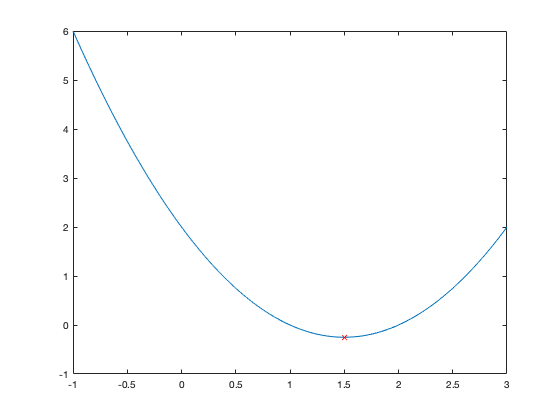
\includegraphics[width=.76\textwidth]{ploti.png}
          \end{center}
        \end{figure}
      \end{proof}
      In this case the algorithm is working in an convex interval, and it starts off at $x_0 = 1$ so we are to the left of the local minium (in this case it is a global one). Every iteration, the computation of the derivative comes out negative so $\alpha_k$ is always positive so in each iteration $x$ increases by .01 approaching the minimizer from the left. 
      \vspace{.15in}

      \item[\textbf{(ii)}]$f(x) = cos(x/50)$
      \begin{proof}[Solution] Running the algorithm on the given $f(x)$\\
        \textbf{Console:}
        \begin{center}
          \lstinputlisting[basicstyle = \footnotesize]{r2.txt}
        \end{center}
        \begin{figure}[H]
          \begin{center}
            \caption{Plotting $f(x)$ with minimum from p8a.}
            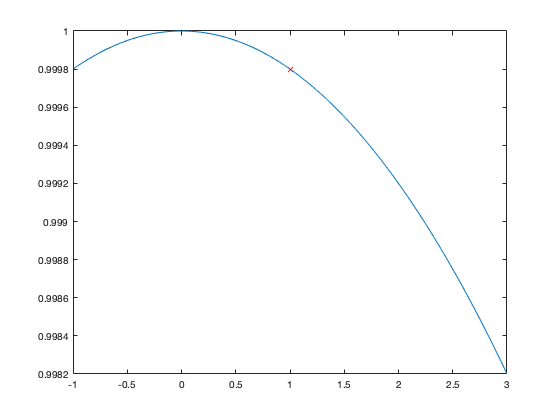
\includegraphics[width=.76\textwidth]{plotii.png}
          \end{center}
        \end{figure}
        Clearly a local minimum will be found to the right of the initial $x_0 = 1$. However since the $df(x_0) < .001$ the 
        algorithm stops on the first iteration and returns the initial point as the minimizer. 
      \end{proof}
      \vspace{.15in}

      \item[\textbf{(iii)}]$f(x) = e^{sin(10x)}$
      \begin{proof}[Solution] Running the algorithm on the given $f(x)$\\
        \textbf{Console:}
        \begin{center}
          \lstinputlisting[basicstyle = \footnotesize]{r3.txt}
        \end{center}
        The algorithm fails to converge, because the step size $\alpha_k$ is too large we end up hopping back and forth around the minimizer. The following plot illustrates this point, note that $f(x)$ is plotted in blue, $f'(x)$ is plotted in red
        and the two points, $x_1 = 1.1$ and $x_2 = 1.09$ are plotted on $f'(x)$ with blue crosses. 
        \begin{figure}[H]
          \begin{center}
            \caption{Plotting $f(x)$, $f'(x)$ and problematic $x_1$ and $x_2$.}
            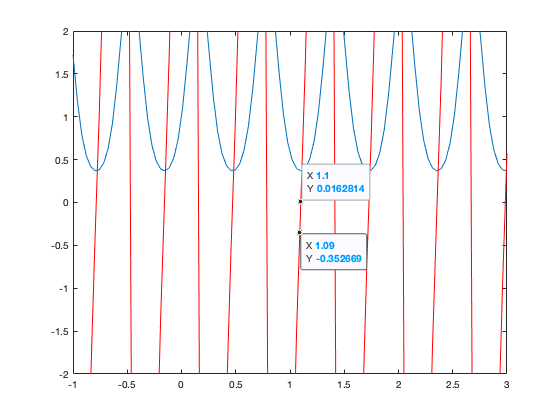
\includegraphics[width=.76\textwidth]{plotiii.png}
          \end{center}
        \end{figure}
      \end{proof}
      \vspace{.15in}

      \item[\textbf{(iv)}]$f(x) = sech(x)$
      \begin{proof}[Solution] Running the algorithm on the given $f(x)$\\
        \textbf{Console:}
        \begin{center}
          \lstinputlisting[basicstyle = \footnotesize]{r4.txt}
        \end{center}
        \begin{figure}[H]
          \begin{center}
            \caption{Plotting $f(x)$ with minimum from p8a.}
            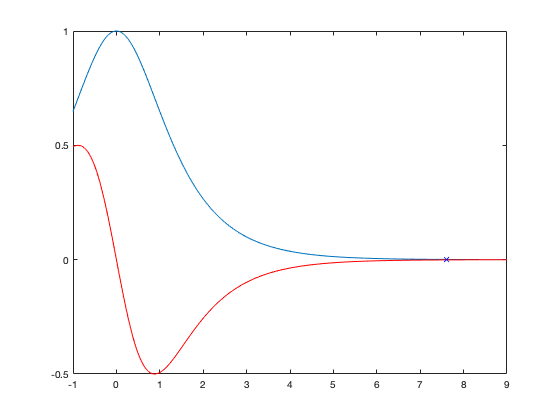
\includegraphics[width=.76\textwidth]{plotiv.png}
          \end{center}
        \end{figure}
        The hyperbolic secant function does not have a global minimum, so this algorithm will continue to add $.01$ to 
        the current iterant until the derivative becomes a value smaller than $.001$. 

      \end{proof}
      \vspace{.15in}
    \end{enumerate}


    \item[\textbf{(c)}] In several complete sentences, describe the main deficiencies of Algorithm P8A. It is a good idea to use the
    results of part \textbf{b} to illustrate some of your points. 
    \begin{proof}[Solution] The main criticisms of this algorithm come from the relatively large stopping criteria, and the fixed step sizes and starting point. Consider \textbf{b(ii)}, with a stopping criteria of $.001$ on the derivative the algorithm couldn't even continue to a second iteration, when clearly if dropped into $f(x) = cos(x/50)$ at $x_0 = 1$ there is a local minimum to the right. Now consider \textbf{b(iii)}, the algorithm was unable to terminate because $\alpha_k$ was too large.

    \end{proof}
    \vspace{.15in}

    \item[\textbf{(d)}] 
    \begin{proof}[Solution] The choice of having $|f'(x_k)| < \epsilon_{machine}$ is the correct one. Any comparison to zero should be made with $\epsilon_{machine}$ instead because of the limits of our double precision arithmetic. Being able to decide on an initial point, will allow us to at least have some say on the runtime, and which local minimizer we converge to. Finally being able to choose a step size will help us avoid situations illustrated in \textbf{b(iii)} where are step size was too small, we get to make the tradeoff between accuracy to the true minimizer and runtime.\\
      This algorithm assumes that the user has some idea about the location of the minimizer on $f(x)$ hence the initial value parameter. It also assumes that the user has some idea of the concavity of $f(x)$, choosing the step size to large for highly concave or convex function will result in a situation like \textbf{b(iii)}. 

    \end{proof}
    \vspace{.15in}
  \end{enumerate}


\end{exercise}
\vspace{.5in}










\end{document}


































